\section{The system description}

\begin{figure}[h!tbp]
\centering
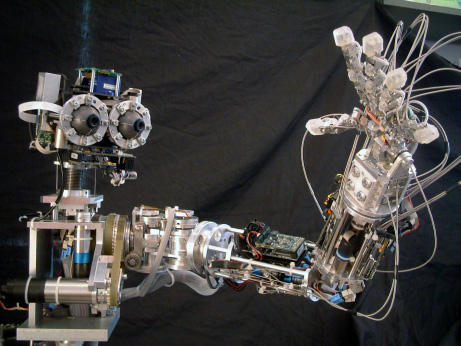
\includegraphics[width=80mm]{Figure/James1.jpg}
\caption{The humanoid robot James.}
\label{Fig:PicureJames}
\end{figure}

The reaching controller has been implemented on our humanoid robot James (see figure \ref{Fig:PicureJames}). James consists of 22 DOFs, actuated by a total of 23 motors, whose torque is transmitted to the joints by belts and stainless-steel tendons. The head is equipped with two eyes, which can pan and tilt independently (4 DOFs), and is mounted on a 3-DOF neck, which allows the movement of the head as needed in the 3D rotational space.


\subsection{Head and eyes actuation structure} \label{Sec:HeadEyesStructure}

\begin{figure}[h!tbp]
  % Requires \usepackage{graphicx}
  \centering
  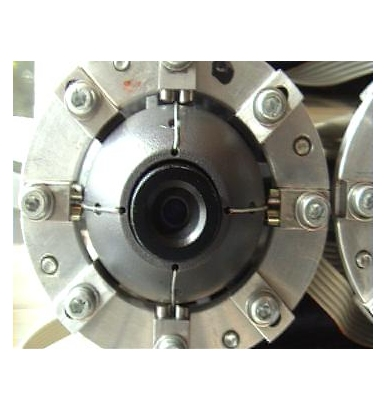
\includegraphics[width=60mm]{Figure/EyePhoto.jpg}
  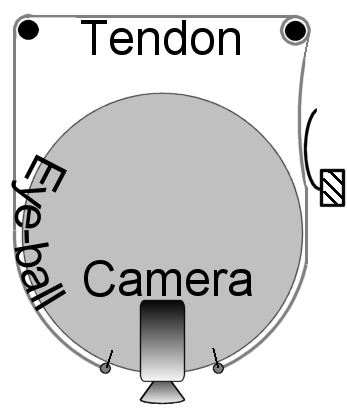
\includegraphics[width=60mm]{Figure/EyeSection.jpg}\\
  \caption{The left picture shows the tendon driven eye. The
 two tendons are actuated by two motors. The first motor moves the vertical
  tendon (tilt motion). The second motor moves the horizontal tendon (pan motion). The
  right figure sketches the actuation scheme.}\label{Fig:EyeSection}
\end{figure}

\begin{figure}
  % Requires \usepackage{graphicx}
  \begin{center}
  \begin{tabular}{ccc}
  \parbox{40mm}{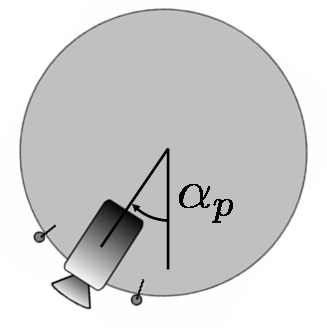
\includegraphics[height=40mm]{Figure/EyePan.jpg}}  & &
  \parbox{40mm}{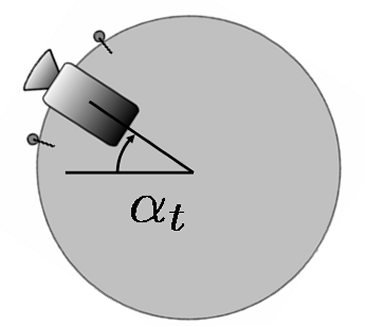
\includegraphics[height=40mm]{Figure/EyeTilt.jpg}}\\
  Top view & & Lateral view
  \end{tabular}
  \end{center}
  \caption{The left picture shows a top view of the eyeball and indicates the pan angle. The right picture instead shows the lateral view with the tilt angle.}\label{Fig:EyePanTilt}
 \end{figure}

\begin{figure}
  % Requires \usepackage{graphicx}
  \begin{center}
  \begin{tabular}{ccc}
  \parbox{60mm}{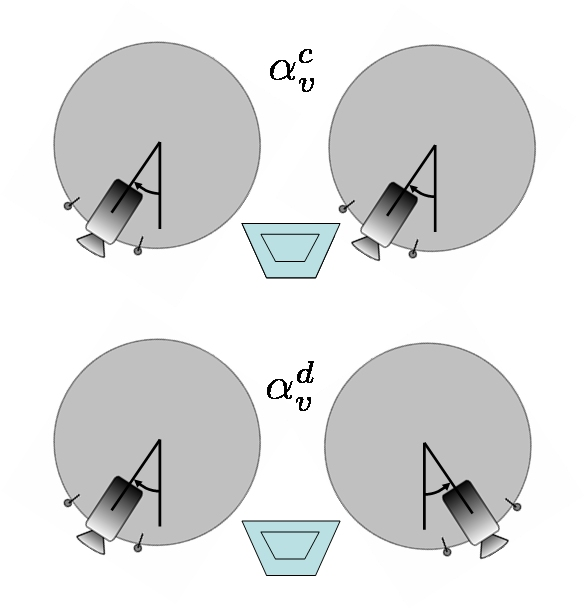
\includegraphics[height=60mm]{Figure/EyeVergenceVersion.jpg}}  & &
  \parbox{60mm}{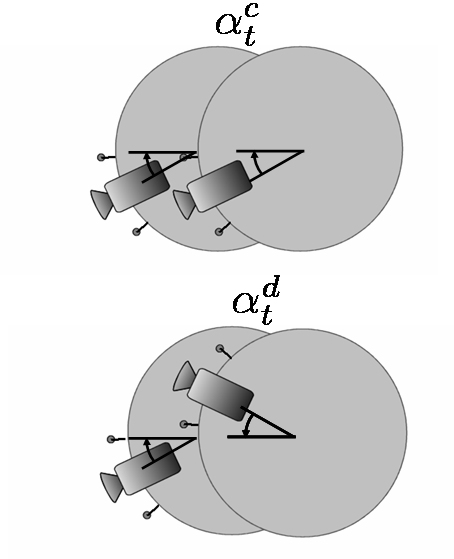
\includegraphics[height=60mm]{Figure/EyeCommDiffTilt.jpg}}\\
  Top view & & Lateral view
  \end{tabular}
  \end{center}
  \caption{The left picture shows a top view of the eyeball and indicates the version (top) and the vergence (down) angles. The right picture instead shows the lateral view with the common (top) and differential tilt (down) angles.}\label{Fig:EyeCoordinatedMovements}
 \end{figure}


The head structure has a total of 7 degrees of freedom, actuated by 8 motors. Four of these motors are used to independently actuate the pan and tilt movements of the left and right eyes (see Figure \ref{Fig:EyeSection} for a scheme of the tendon actuation). The following notation will be used from now on:
\begin{align*}
\alpha_t^r & \mbox{ : } \mbox{right eye tilt} & \alpha_p^r & \mbox{ : } \mbox{right eye pan}\\
\alpha_t^l & \mbox{ : } \mbox{left eye tilt} & \alpha_p^l & \mbox{ : } \mbox{left eye pan}
\end{align*}
Even though the eyes can be moved independently, our strategy was to couple their movements so as to achieve a more human-like motion. In particular, instead of controlling $\alpha_t^r$, $\alpha_p^r$, $\alpha_t^l$, $\alpha_p^l$ we decided to use vergence $\alpha_v^d$, version $\alpha_v^c$, common tilt $\alpha_t^c$ and differential tilt $\alpha_t^d$ defined as follows:
\begin{align*}
\alpha_v^d & = \frac{\alpha_p^r - \alpha_p^l}{2} & \alpha_v^c & = \frac{\alpha_p^r + \alpha_p^l}{2},\\
\alpha_t^d & = \frac{\alpha_p^r - \alpha_p^l}{2} & \alpha_t^c & = \frac{\alpha_p^r + \alpha_p^l}{2}.
\end{align*}
Practically, the differential tilt angle will not be used. The underlying assumption is the perfect orthogonality between the camera axis and the pan axis of rotation\footnote{\samepage Suppose that our task consists in fixating a given target, i.e. putting the target projections in the center of the left and right image planes. Since the target moves in a three dimensional space, in principle we only need three control variables to actually fixate the target in every possible configuration. It can be shown that these three variables can be $\alpha_v^d$, $\alpha_v^c$ and $\alpha_t^c$ (while keeping $\alpha_t^d=0$) if the system mechanics and optics are perfectly aligned. In particular, the assumptions are the following:
\begin{enumerate}
\item the cameras behave as a perfect pin-hole camera model,
\item the cameras optical axes are orthogonal to the corresponding pan axes of rotation,
\item the pan axes are orthogonal if $\alpha_t^d=0$.
\end{enumerate}}. Practically, the eyes configuration will be denoted $\mathbf q_{eyes} = \begin{bmatrix} \alpha_v^d & \alpha_v^c & \alpha_t^c \end{bmatrix}^\top \in \mathbb R^3$.


The neck actuation is also non conventional. One motor directly actuates the head yaw, denoted $\theta_y$. The remaining three motors actuate the two additional rotations of the head: head pitch $\theta_p$ and head roll $\theta_r$. These two rotations are achieved with an unconventional actuation structure (see Figure \ref{Fig:Head}). Each motor pulls a tendon; the tension of the three tendons determines the equilibrium configuration of the spring on which the head is mounted. The structure has an implicit compliance but it can become fairly stiff when needed by pulling the three tendons simultaneously. The total head configuration (excluding the eyes) will be denoted $\mathbf q_{neck} = \begin{bmatrix} \theta_y & \theta_p & \theta_r \end{bmatrix}^\top \in \mathbb R^3$.

\begin{figure}[tbp]
\centering
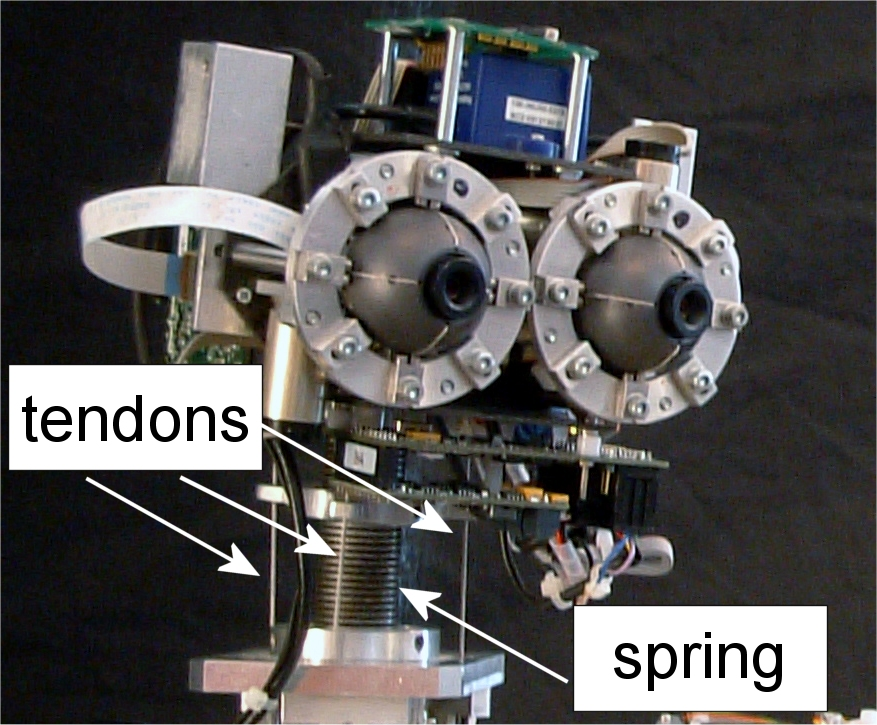
\includegraphics[width=80mm]{Figure/Head.jpg}
\caption{The pictures describes the neck actuation. Practically, the head is mounted on a spring. The spring is moved by pushing and pulling three tendons by the use of conventional DC motors.}
\label{Fig:Head}
\end{figure}

